\documentclass[a4paper]{article}
\usepackage{amsfonts}
\usepackage{amsmath}
\usepackage{amssymb}
\usepackage{graphicx}
\newcommand{\dint}{\displaystyle\int}     

\begin{document}
  
\noindent \large Auteur: Etienne El Hachem \\
\noindent \large Studierichting: Informatica\\
\noindent \large Oefeningenreeks 5D nr. 2.3\\

\medskip

\normalsize

$f(x) = \ln x$

Voor [1,2]:\\

$\dint\limits_1^2 \ln x dx = \left[x\cdot\ln x - x\right]_1^2 = 2\ln2-2+1 = 2\ln2 - 1$\\

Voor [1,e]:\\

$\dint\limits_1^e \ln xdx = \left[x\cdot\ln x - x\right]_1^e = 0 + 1 = 1$\\

\begin{figure}[h]
\centering
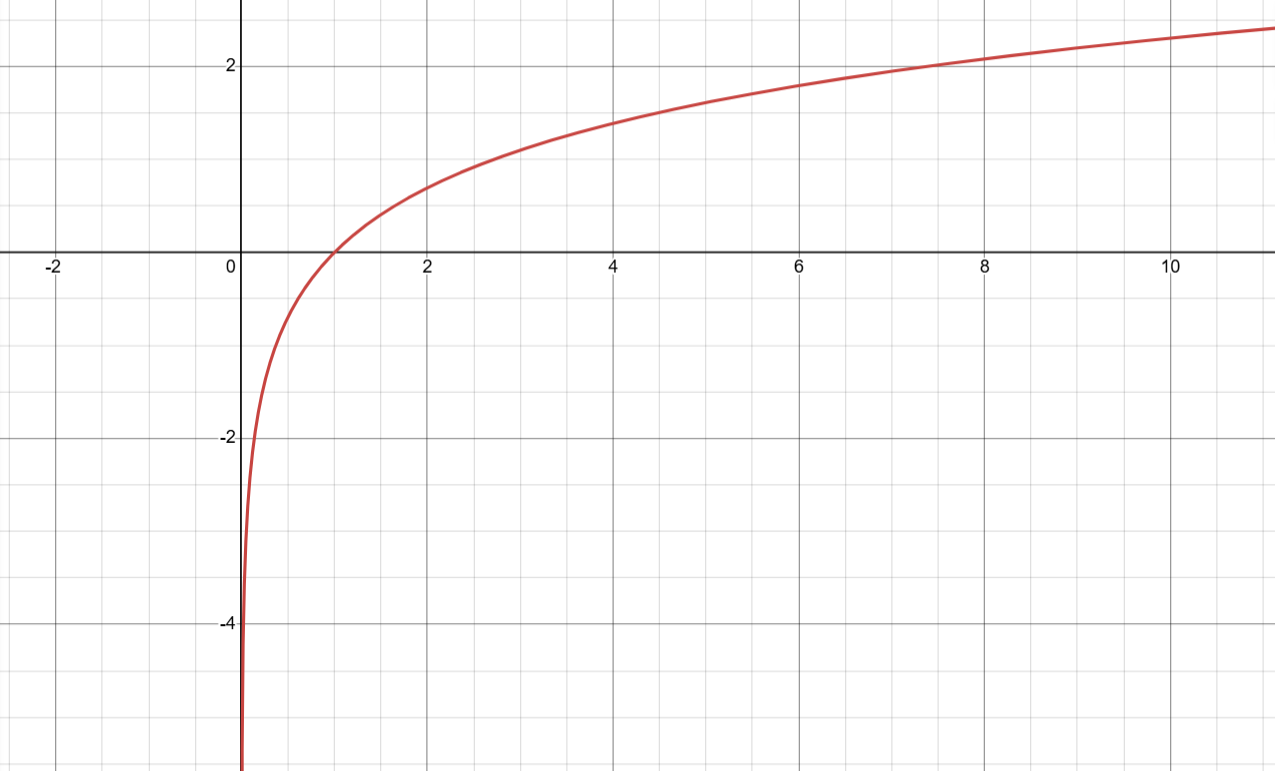
\includegraphics[width=5cm]{5D-2.3-etienne.el.hachem.INF.png}
\end{figure}

\begin{thebibliography}{999}
%\bibitem{a} Referentie
\end{thebibliography}
\end{document} 
